\documentclass[compress,aspectratio=169]{beamer}
\usepackage{ragged2e}
\usepackage{underscore}
%Setup File
% \usepackage[english]{babel}
\usepackage[brazilian]{babel}
\usepackage[letterpaper,top=2cm,bottom=2cm,left=3cm,right=3cm,marginparwidth=1.75cm]{geometry}

% Useful packages
\usepackage{amsmath}
\usepackage{graphicx}
% \usepackage[colorlinks=true,linkcolor=blue]{hyperref}
\usepackage{hyperref}
\usepackage{listings}
\usepackage[figure,table,lstlisting]{totalcount}
\usepackage{tcolorbox}
\usepackage{listings}
\usepackage{xcolor}
\usepackage{setspace}
\usepackage{float} 
\usepackage[numbers]{natbib}



\hypersetup{
    colorlinks=true,
    linkcolor=black,
    filecolor=magenta,      
    urlcolor=cyan,
    pdftitle={Trabalho pratico de projeto e analise de algoritmos},
    pdfpagemode=FullScreen,
    }

\definecolor{verde}{rgb}{0.25,0.5,0.35}
\definecolor{jpurple}{rgb}{0.5,0,0.35}

\lstset{
  language=C++,
  basicstyle=\ttfamily\small,
  keywordstyle=\color{jpurple}\bfseries,
  stringstyle=\color{red},
  commentstyle=\color{verde},
  morecomment=[s][\color{blue}]{/**}{*/},
  extendedchars=true,
  showspaces=false,
  showstringspaces=false,
  numbers=left,
  numberstyle=\tiny,
  breaklines=true,
  backgroundcolor=\color{cyan!10},
  breakautoindent=true,
  captionpos=b,
  xleftmargin=0pt,
  tabsize=4
}

\renewcommand{\lstlistingname}{Código}
\renewcommand{\lstlistlistingname}{Lista de Códigos Fonte}

\newcommand\conditionalLoF{%
    \iftotalfigures
        \listoffigures
    \fi}
\newcommand\conditionalLoT{%
    \iftotaltables
        \listoftables
    \fi}
\newcommand\conditionalLoL{%
    \iftotallstlistings
        \lstlistoflistings
    \fi}

\newcommand{\DESCRICAO}[1]{
    % set flexible interword space
    \setlength{\spaceskip}{0.5em plus 1em minus 0.1em}%
    % add some space with not as much flexibility, but only
    % if some space precedes
    \ifdim\lastskip>0pt \hspace{0.5em plus 0.5em minus 0.1em}\fi
    \texttt{\textbf{\color{red}#1}}
}

\newcommand{\CAPA}[4]{
    % 1) Título
    % 2)
    % 3)
    % 4)
    \begin{titlepage}
    	
    	  \vfill
    	
    	  \begin{center}
    	    \begin{large}
    	      Universidade Federal de Ouro Preto - UFOP
    	    \end{large}
    	  \end{center}
    	
    	  \begin{center}
    	    \begin{large}
    	      Instituto de Ciências Exatas e Biológicas - ICEB
    	    \end{large}
    	  \end{center}
    	
    	  \begin{center}
    	    \begin{large}
    	      Departamento de Computação - DECOM
    	    \end{large}
    	  \end{center}
          
          \begin{center}
    	    \begin{large}
              Ciência da Computação
    	    \end{large}
    	  \end{center}
    	  
    	  \vfill
          \vfill
    	
    	  \begin{center}
    	    \begin{Huge}
    	      #1\\
    	    \end{Huge}
    	    \begin{Large}
              #2\\
    	    \end{Large}
    	  \end{center}
    	  
    	  \vfill
    	  
    	  \begin{center}
    	    \begin{large}
              #3
    	    \end{large}
    	  \end{center}
    	
    	  \begin{center}
    	    \begin{large}
    	      Professor: #4
    	    \end{large}
    	  \end{center}
    	
    	  \vfill
          \vfill
    	
    	  \begin{center}
    	    \begin{large}
    	      Ouro Preto \\
    	      \today \\
    	    \end{large}
    	  \end{center}    
    
    
    \clearpage
    \newpage

    \tableofcontents
    \conditionalLoF
    \conditionalLoT
    \conditionalLoL
	
    % \thispagestyle{empty}
    % \tableofcontents
    % \newpage
    % \thispagestyle{empty}
    
    % \listoffigures
    
    % \lstlistoflistings
    % \newpage
    % \thispagestyle{empty}
    \end{titlepage}
}
\addbibresource{setup/refs.bib}


\subtitle[PAA]  {Clique, Conjunto Independente e SAT}
\begin{document}
\begindocument

\section{Introdução}
    \begin{frame}{Clique, Conjunto indpendente e SAT}
        \begin{justify}
            \begin{itemize}
                \item A Satisfabilidade, ou SAT, é um problema de grande importância prática, com aplicações em diversas áreas, como teste de circuitos e design de software.
                \item O problema do clique consiste em encontrar um subgrafo completo em que todos vértices estão conextados entre si, sendo um desafio NP-completo com aplicações em várias áreas.
                \item O problema do conjunto indpendente pode ser reduzido ao problema do Clique, pois um conjunto de nós que forma um Conjunto Independente em um grafo é equivalente a um conjunto que forma um Clique em seu grafo complementar.
            \end{itemize}
        \end{justify}
    \end{frame}


\section{Clique}
    \begin{frame}{Problema do Clique}
        \begin{justify}
            Dado um grafo, o objetivo é encontrar um conjunto máximo de vértices tal que todas as possíveis arestas entre eles estejam presentes. Para isso, foi utilizado a estratégia \textit{branch and bound} para encontrar a solução do problema.
        \end{justify}
    \end{frame}
    
    \begin{frame}{Definição do problema}
        \begin{itemize}
            \item \textbf{Variáveis para a solução:} \(X_1, \dots, X_n\), onde \(X_i\) representa um vértice pertencente ao grafo.
            \item \textbf{Domínio para as variáveis da solução:} \{0, 1\}, onde 0 indica que aquele vértice não faz parte do clique máximo e 1 indica o contrário.
            \item \textbf{Restrições:} Todos os vértices representados pelas variáveis que possuem valor 1 devem estar conectados entre si através de uma aresta.
            \item \textbf{Objetivo:} Obter o maior conjunto possível de vértices tal que todas as possíveis arestas entre eles estejam presentes.
        \end{itemize}
    \end{frame}

    \begin{frame}{Leitura do Problema}
        \begin{itemize}
            \item O problema foi lido e armazenado em uma única variável, contendo o número de vértices e a matriz de adjacência do grafo.
            \item O vetor que armazena a solução inicial foi iniciado com todas as posições possuindo valores -1, para representar que a mesma começa vazia.
        \end{itemize}
    \end{frame}

    \begin{frame}[fragile]{Geração Inicial da Melhor Solução}
        \begin{lstlisting}
def geraSolucao(problema):
    solucao = [0] * problema[0][0]

    for i in range(problema[0][0]):
        for j in range(problema[0][0]):
            if(problema[i+1][j] == 1):
                solucao[i] = 1
                solucao[j] = 1
                return solucao

    solucao[0] = 1
    return solucao
        \end{lstlisting}
    \end{frame}
    
    \begin{frame}[fragile]{Função que executa o branch and bound}
        \begin{lstlisting}
def branchAndBoundClique(solucao, i, problema, melhor):
    if eCompleta(solucao, problema):
        melhor[:] = solucao
        return melhor
    
    else:
        for j in range(2):
            solucao[i] = j
            
            if(eConsistente(solucao, problema, i) and ePromissora(solucao, problema, melhor, i)):
                melhor = branchAndBoundClique(solucao, i+1, problema, melhor)
            
            solucao[i] = -1
        
        return melhor
        \end{lstlisting}
    \end{frame}

    \begin{frame}[fragile]{Função que verifica a consistência da solução}
        \begin{lstlisting}
def eConsistente(solucao, problema, i):
    verticesNaSolucao = []
    
    for j in range(i+1):
        if solucao[j] == 1:
            verticesNaSolucao.append(j)

    for j in range(len(verticesNaSolucao)-1):
        for k in range(j+1, len(verticesNaSolucao)):
            if(problema[verticesNaSolucao[j]+1][verticesNaSolucao[k]] == 0):
                return False
            
    return True 
        \end{lstlisting}
    \end{frame}

    \begin{frame}[fragile]{Função que verifica se a solução é promissora}
        \begin{lstlisting}
def ePromissora(solucao, problema, melhor, i):
    numVerticesMelhor = sum(melhor)
    numVerticesMaximoSolucao = 0 # armazena o numero maximo de vertices possiveis nessa solucao
    
    for j in range(i+1):
        numVerticesMaximoSolucao += solucao[j]

    numVerticesMaximoSolucao += (problema[0][0] - (i+1))
    
    return numVerticesMaximoSolucao > numVerticesMelhor
        \end{lstlisting}
    \end{frame}

    \begin{frame}
        \begin{figure}[H]
            \centering
            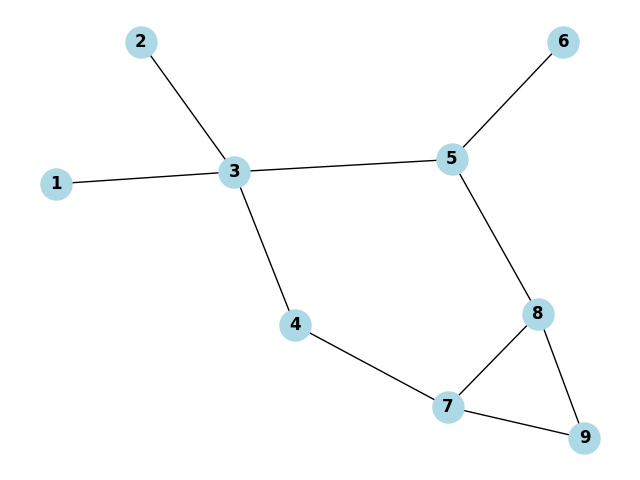
\includegraphics[width=0.65\textwidth]{images/grafo_instancia1.png}
            \caption{Grafo da instância de entrada.}
            \label{fig:instancia1Clique}
        \end{figure}
    \end{frame} 

    \begin{frame}
        \begin{tcolorbox}[title=Saída da instância de entrada, width=\linewidth, 
          fontupper=\ttfamily, 
          halign=flush left]
            [0, 0, 0, 0, 0, 0, 1, 1, 1] \\
            Vértices presentes no clique: \\
            7 \\
            8 \\
            9 \\
            Tempo de execução: 0.001000 segundos \\
        \end{tcolorbox}
    \end{frame}

\section{Conjunto Independente}
    \begin{frame}{O problema do Conjunto Independente}
    \begin{justify}
        Para resolver o problema do Conjunto Independente (ou Conjunto Estável) por meio de uma redução polinomial ao problema do Clique, iremos usar a relação entre esses dois problemas. Sabemos que um conjunto independente de um grafo é equivalente a um clique no complemento desse grafo.
    \end{justify}
    \end{frame}

    \begin{frame}{Passos para a solução}
        \begin{itemize}
            \item \textbf{Complemento do grafo:} O complemento de um grafo é um grafo onde as arestas que estavam presentes no grafo original são removidas e as arestas que não estavam presentes são adicionadas.
            \item \textbf{Redução:} Dado um grafo GGG, o problema do conjunto independente em GGG pode ser resolvido encontrandoo o clique máximo no complemento do grafo G'G'G'.
            \item \textbf{Aproveitar a implementação do clique:} Após calcular o complemento do grafo, aplicamos o algoritmo de clique já implementado.\\
        \end{itemize}
    \end{frame}

    \begin{frame}[fragile]{Função geraComplemento}
        \begin{lstlisting}
def geraComplemento(problema):
    numVertices = problema[0][0]  # Numero de vertices (primeira linha da matriz)
    
    # Inicializa a matriz de complemento
    complemento = [[0] * numVertices for _ in range(numVertices)]
    
    # Preenche a matriz de complemento
    for i in range(numVertices):
        for j in range(numVertices):
            if i != j:  # Nao considerar a diagonal principal
                complemento[i][j] = 1 - problema[i + 1][j]
    
    # Adiciona o numero de vertices como a primeira linha da matriz de complemento
    complemento.insert(0, [numVertices])
    
    return complemento
        \end{lstlisting}
    \end{frame}
    \begin{frame}
        \begin{figure}[H]
            \centering
            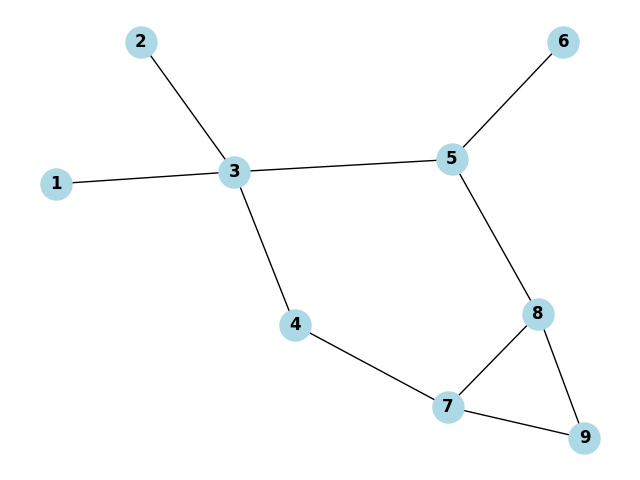
\includegraphics[width=0.65\textwidth]{images/grafo_instancia1.png}
            \caption{Grafo da instância de entrada.}
            \label{fig:instancia1}
        \end{figure}
    \end{frame} 

    \begin{frame}
        \begin{figure}[H]
            \centering
            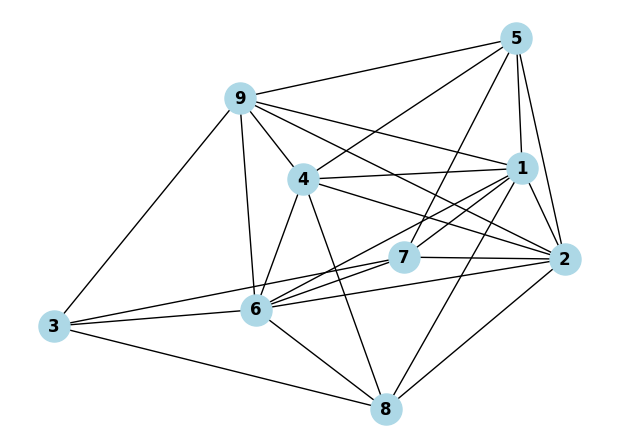
\includegraphics[width=0.65\textwidth]{images/conj_instancia1.png}
            \caption{Grafo complemento da instância de entrada.}
            \label{fig:instancia2}
        \end{figure}
    \end{frame}
    
    \begin{frame}{Saída}
        \begin{tcolorbox}[title=Saída da instância, width=\linewidth, 
          fontupper=\ttfamily, 
          halign=flush left]
            Conjunto independente máximo: {1, 2, 4, 6, 9}\\
            Tempo de execução: 0.002493 segundos\\
        \end{tcolorbox}
    \end{frame}

\section{SAT}
    \begin{frame}{O problema SAT}
        \begin{justify}
            Dada uma fórmula booleana na forma normal conjuntiva, é necessário encontrar, com \textit{backtracking}, algum resultado que satisfaça a mesma. 
            Caso não seja possível, informa tal possibilidade
        \end{justify}
    \end{frame}
    \begin{frame}{Definição do problema}
        \begin{itemize}
            \item \textbf{Variáveis para a solução:} \(X_1, \dots, X_n\), onde \(X_i\) indica o valor verdade para determinada variável do problema;
            \item \textbf{Domínio para as variáveis da solução:} \{False, True\};
            \item \textbf{Restrições:} Todas as cláusulas devem resultar em verdadeiro
            \item \textbf{Objetivo:} Obter algum conjunto de valores do domínio para as variáveis de forma que todas as cláusulas sejam satisfeitas
        \end{itemize}
    \end{frame}
    \begin{frame}{Entrada}
        \[(A \lor \neg B \lor C) \land (\neg A \lor B \lor D) \land (B \lor \neg C \lor \neg D) \land (\neg A \lor \neg B \lor D)\]
        \begin{tcolorbox}[title=Arquivo de entrada para a fórmula, width=\linewidth, fontupper=\ttfamily, halign=flush left]
            4 \\
            1 0 1 -1 \\
            0 1 -1 1 \\
            -1 1 0 0 \\
            0 0 -1 1
        \end{tcolorbox}
    \end{frame}

    \begin{frame}[fragile]{Backtracking}
        \begin{lstlisting}
def backtrack(solucao, i, problema):
    dominio = [False, True]
    if verificar_solucao(problema, solucao):
        return True
    else:
        i = i + 1
        candidatos = construir_candidatos(solucao, i, problema, dominio)
        for c in candidatos:
            solucao[i-1] = c
            finished = backtrack(solucao, i, problema)
            if finished:
                return True
            solucao[i-1] = None
    return False
        \end{lstlisting}
    \end{frame}

    \begin{frame}{Construir candidatos}
        \begin{itemize}
            \item Iterar sobre cada valor do domínio e colocá-lo na solução
            \item Verificar cada cláusula do problema
            \item Verificar se as variáveis já atribuídas compõem a cláusula
            \item Se comporem, verificar se a cláusula é satisfeita. 
            \item Se todas as cláusulas forem satisfeitas, o valor pode ser suficiente.
            \item Se uma cláusula não for, tal valor do domínio não poderá participar da solução.
        \end{itemize}
    \end{frame}

    \begin{frame}[fragile]{Construir candidatos}
        \begin{lstlisting}
def construir_candidatos(solucao, i, problema, dominio):
    if i > len(solucao): return []
    candidatos = dominio.copy()
    s_temp = solucao.copy()
    qtd_variaveis = len(problema[0])
    for c in dominio:
        s_temp[i-1] = c
        for clausula in problema:
            satisfeita = False  
            if clausula_computavel(i, clausula, qtd_variaveis):
                for variavel_atual, literal in enumerate(clausula):
                    if literal == 1:
                        satisfeita = satisfeita or s_temp[variavel_atual]
                    elif literal == 0:
                        satisfeita = satisfeita or not s_temp[variavel_atual]
            else:continue
            if not satisfeita:
                candidatos.pop(0)
                break
    return candidatos
        \end{lstlisting}
    \end{frame}

    \begin{frame}[fragile]{Cláusula computável}
        \begin{itemize}
            \item A cláusula a seguir não poderá ser computável.
            \item Estamos analisando o valor do True e a cláusula ficará falsa.
            \item Não sabemos se ela será verdadeira ou falsa no fim do processamento.
        \end{itemize}
        \begin{tcolorbox}[width=\linewidth, fontupper=\ttfamily,  halign=flush left]
            Cláusula: 1 -1 0 0 1 \newline 
            Solução: [False, False, True, \_, \_] \newline
            i = 3
        \end{tcolorbox}
        \begin{lstlisting}
def clausula_computavel(i, clausula, qtd_variaveis):  
    for j in range(i, qtd_variaveis):
        if clausula[j-1] == -1:
            return False
        \end{lstlisting}
    \end{frame}


    \begin{frame}{Exemplo instância}
        \[(A \lor B \lor C) \land (A \lor \neg B) \land (B \lor \neg C) \land (\neg A \lor C) \land (\neg A \lor \neg B \lor \neg C)\]
        
        \begin{tcolorbox}[title=Saída da instância, width=\linewidth, fontupper=\ttfamily, halign=flush left]
            Solução não encontrada \\
            Tempo de execução: 0.000503 segundos \\  
        \end{tcolorbox}
    \end{frame}
    %%%%%%%%%%%%%%%%%%%%%%%%%%%%%%%%%%%%%%%%%%%%%%
    \begin{frame}{Exemplo instância}
        \begin{center}
            \((A \lor B \lor C) \land (\neg A \lor \neg B \lor \neg C) \land (A \lor \neg B \lor D) \land (\neg A \lor B \lor \neg D) \land (A \lor \neg C \lor D) \land \)

            \((\neg A \lor C \lor \neg D) \land (\neg A \lor \neg B \lor C \lor D) \land (A \lor B \lor \neg C \lor \neg D)\)
            
        \end{center}
        
        \begin{tcolorbox}[title=Saída da instância, width=\linewidth, fontupper=\ttfamily, halign=flush left]
            Solução encontrada: [False, True, False, True] \\
            Tempo de execução: 0.000151 segundos
        \end{tcolorbox}
    \end{frame}


\section{Referências}
\begin{frame}{Referências utilizadas}
    
    \begin{justify}
        \begin{itemize}
           \item MANOLOPOULOS, Y.; NANOPOULOS, A.; PAPADOPOULOS, A. N.; THEODORIDIS, Y. R-Trees: Theory and Applications. Springer, 2006. 
           \item KAO, M.-Y. Encyclopedia of Algorithms. Springer, 2008.
           \item Introduction to R tree. GeeksforGeeks. Disponível em: <https://www.geeksforgeeks.org/introduction-to-r-tree/>. Acesso em: 17 ago. 2023.
           \item WIKIPEDIA CONTRIBUTORS. R-tree. Wikipedia. Disponível em: <https://en.wikipedia.org/wiki/R-tree>. Acesso em: 17 ago. 2023.
        \end{itemize}
    \end{justify}
\end{frame}



\end{document}
